
%(BEGIN_QUESTION)
% Copyright 2003, Tony R. Kuphaldt, released under the Creative Commons Attribution License (v 1.0)
% This means you may do almost anything with this work of mine, so long as you give me proper credit

The metal case of this appliance is {\it grounded} by means of a third conductor:

$$\includegraphics[width=15.5cm]{i02411x01.eps}$$

Explain how this grounding connection makes the appliance safer for anyone touching its metal case.  Also, explain why both the fuse and the power switch are intentionally placed in series with the {\it ungrounded} (``hot'') power conductor.

\underbar{file i02411}
%(END_QUESTION)





%(BEGIN_ANSWER)

The ground wire connection makes the metal case of the appliance electrically common with earth ground.

%(END_ANSWER)





%(BEGIN_NOTES)

Ask your students to explain why the case's electrical commonality with earth makes it safer to touch.  What do they know about ``electrically common points'' in a circuit, and voltage between those points?

\vskip 10pt

The placement of the fuse and switch in series with the hot conductor is for the purpose of disconnecting the most dangerous wire from the device in the event of overcurrent (fuse blowing) or intentional shutdown (power switch turning off).

%INDEX% Electronics review: safety grounding of electrical devices

%(END_NOTES)


